\documentclass{article}
\usepackage{cmap}
\usepackage[utf8]{inputenc}
\usepackage[english,ukrainian]{babel}
\usepackage{graphicx}
\usepackage{geometry}
\usepackage{listings}
\usepackage{float}
\usepackage{amsmath}
\geometry{
	a4paper,
	left=20mm,
	right=20mm,
	top=15mm,
	bottom=15mm,
}
\lstset{
	language=c,
	tabsize=4,
	keepspaces,
	showstringspaces=false,
}
\graphicspath{ {./pictures} }
\setlength{\parindent}{4em}

\newcommand\subject{Основи електроніки}
\newcommand\lecturer{професор кафедри ПЗ \\ Фечан А.В.}
\newcommand\teacher{доцент кафедри ПЗ \\ Коцун В.І.}
\newcommand\mygroup{ПЗ-22}
\newcommand\lab{3}
\newcommand\theme{Аналіз перехідних процесів у колах із зосередженими
	параметрами засобами програмного продукту Multisim Live}
\newcommand\purpose{Навчитись аналізувати перехідні процеси у колах із зосередженими
	параметрами засобами програмного продукту Multisim Live}

\begin{document}
\begin{normalsize}
	\begin{titlepage}
		\thispagestyle{empty}
		\begin{center}
			\textbf{МІНІСТЕРСТВО ОСВІТИ І НАУКИ УКРАЇНИ\\
				НАЦІОНАЛЬНИЙ УНІВЕРСИТЕТ "ЛЬВІВСЬКА ПОЛІТЕХНІКА"}
		\end{center}
		\begin{flushright}
			\textbf{ІКНІ}\\
			Кафедра \textbf{ПЗ}
		\end{flushright}
		\vspace{200pt}
		\begin{center}
			\textbf{ЗВІТ}\\
			\vspace{10pt}
			до лабораторної роботи № \lab\\
			\textbf{на тему}: “\textit{\theme}”\\
			\textbf{з дисципліни}: “\subject”
		\end{center}
		\vspace{112pt}
		\begin{flushright}
			
			\textbf{Лектор}:\\
			\lecturer\\
			\vspace{28pt}
			\textbf{Виконав}:\\
			
			студент групи \mygroup\\
			Коваленко Д.М.\\
			\vspace{28pt}
			\textbf{Прийняв}:\\
			
			\teacher\\
			
			\vspace{28pt}
			«\rule{1cm}{0.15mm}» \rule{1.5cm}{0.15mm} 2023 р.\\
			$\sum$ = \rule{1cm}{0.15mm}……………\\
			
		\end{flushright}
		\vspace{\fill}
		\begin{center}
			\textbf{Львів — 2023}
		\end{center}
	\end{titlepage}
		
	\begin{description}
		\item[Тема.] \theme.
		\item[Мета.] \purpose.
	\end{description}

	\section*{Теоретичні відомості}

	
		\section*{Індивідуальне завдання}
	\begin{enumerate}
		\item Згідно отриманого завдання провести аналіз перехідних процесів в не
		розгалуженому колі змінного струму (для знаходження величин L та C
		прийняти за робочою частотою схеми 1кГц).
		\item Відтворити схему в середовищі Multisim Live та запустити її симуляцію.
		\item Побудувати часові залежності струмів та напруг схеми.
		\item Провести аналіз параметрів кола визначити тривалість перехідних
		процесів та максимальне відхилення струмів та напруг схеми в порівнянні
		з стаціонарними значеннями.
	\end{enumerate}
	
	\begin{figure}[H]
		\centering
		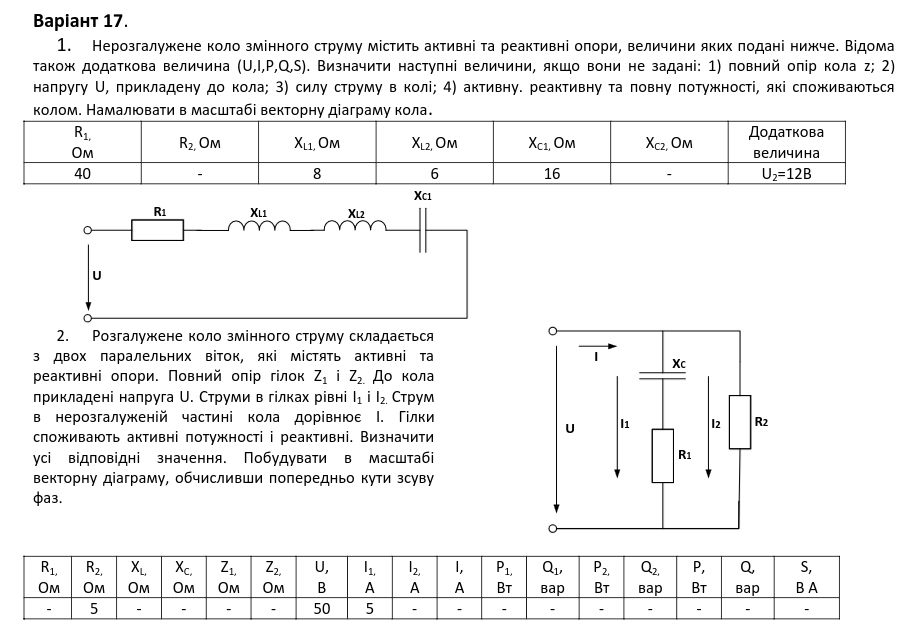
\includegraphics[scale=0.5]{v}
	\end{figure}
	
	\section*{Хід виконання}
	\begin{figure}[H]
		\centering
		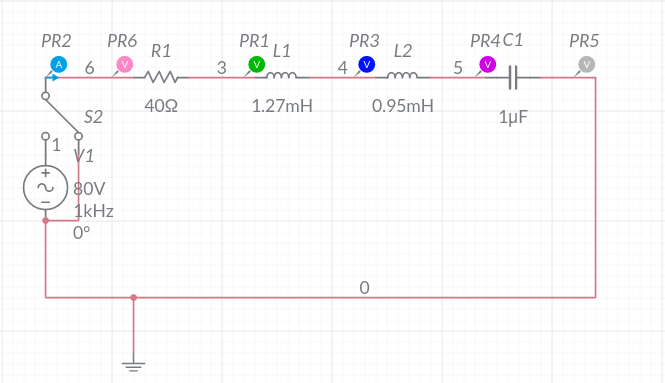
\includegraphics[scale=0.5]{s}
		\caption{Відтворив схему нерозгалуженого кола змінного стуму в середовищі Multisim Live.}
	\end{figure}
	
	\begin{figure}[H]
		\begin{minipage}[t]{0.45\textwidth}
			\centering
			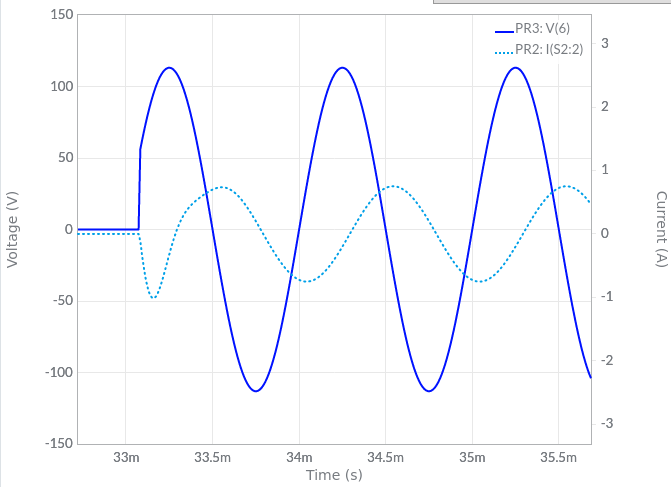
\includegraphics[width=\textwidth]{11}
		\end{minipage}
		\hfill
		\begin{minipage}[t]{0.45\textwidth}
			\centering
			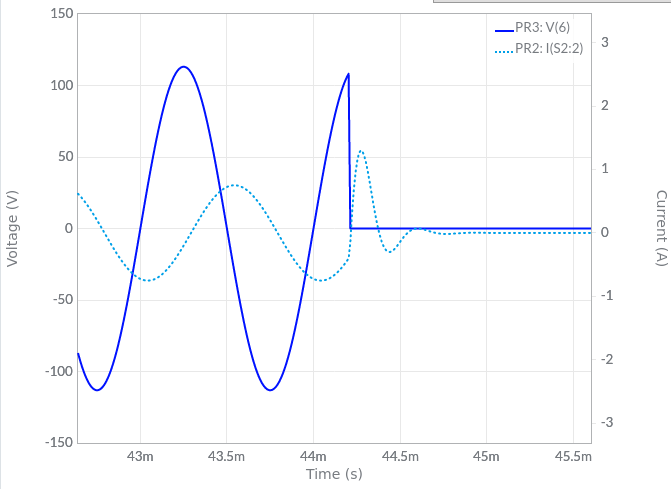
\includegraphics[width=\textwidth]{12}
		\end{minipage}
		\caption{Перехідний процес на резисторі.}
	\end{figure}
	
	\begin{figure}[H]
		\begin{minipage}[t]{0.45\textwidth}
			\centering
			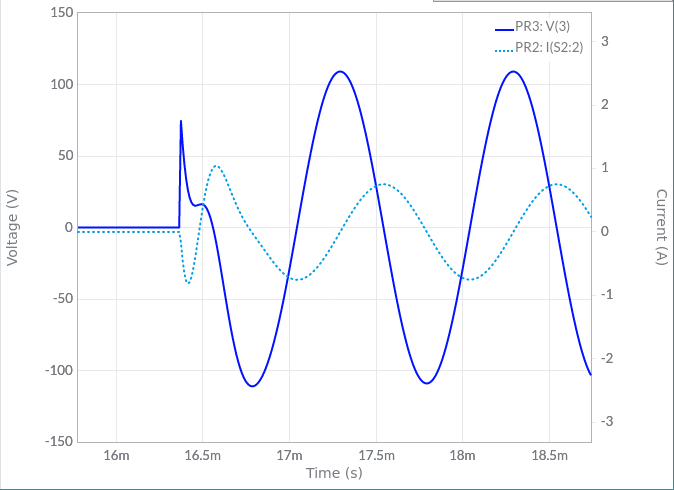
\includegraphics[width=\textwidth]{21}
		\end{minipage}
		\hfill
		\begin{minipage}[t]{0.45\textwidth}
			\centering
			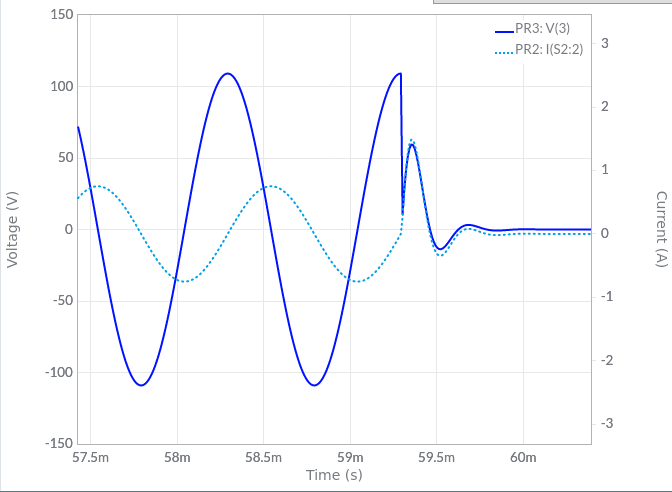
\includegraphics[width=\textwidth]{22}
		\end{minipage}
		\caption{Перехідний процес на котушці №1.}
	\end{figure}

	\begin{figure}[H]
		\begin{minipage}[t]{0.45\textwidth}
			\centering
			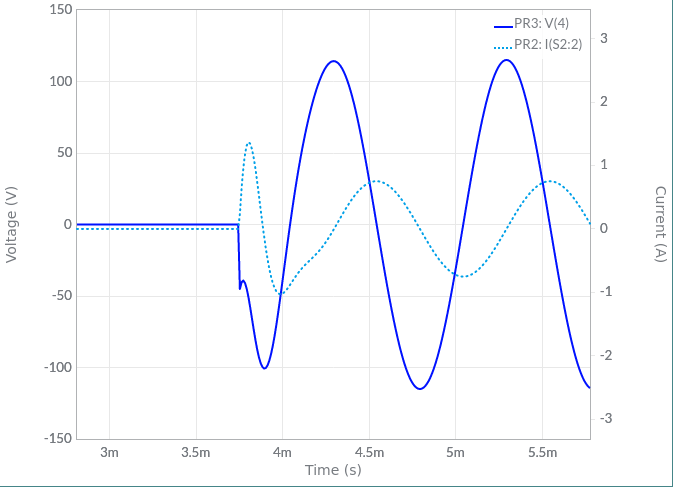
\includegraphics[width=\textwidth]{31}
		\end{minipage}
		\hfill
		\begin{minipage}[t]{0.45\textwidth}
			\centering
			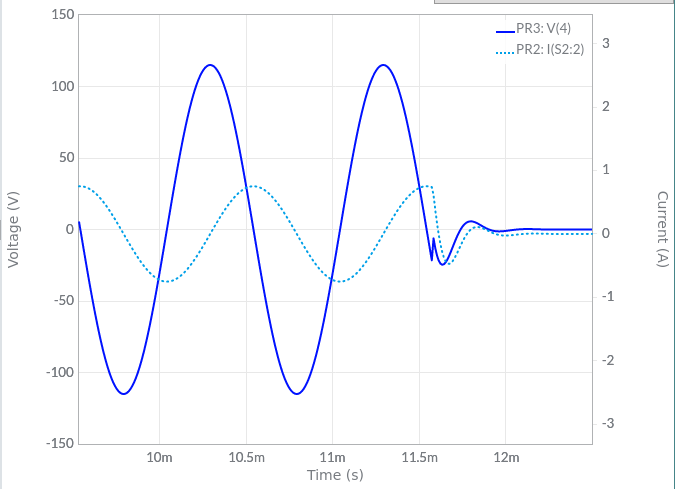
\includegraphics[width=\textwidth]{32}
		\end{minipage}
		\caption{Перехідний процес на котушці №2.}
	\end{figure}
	
	\begin{figure}[H]
		\begin{minipage}[t]{0.45\textwidth}
			\centering
			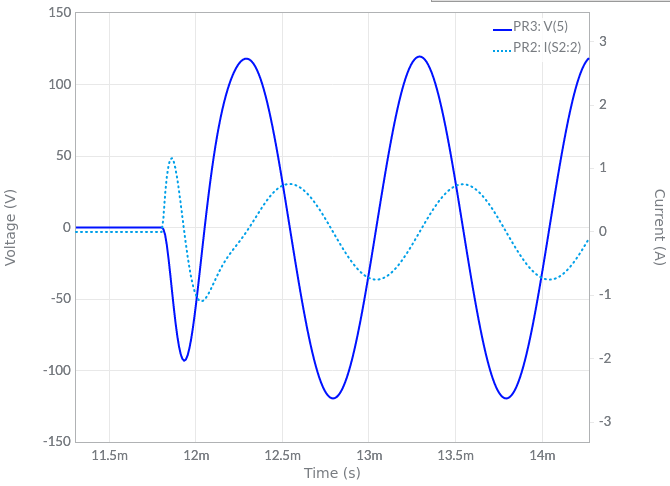
\includegraphics[width=\textwidth]{41}
		\end{minipage}
		\hfill
		\begin{minipage}[t]{0.45\textwidth}
			\centering
			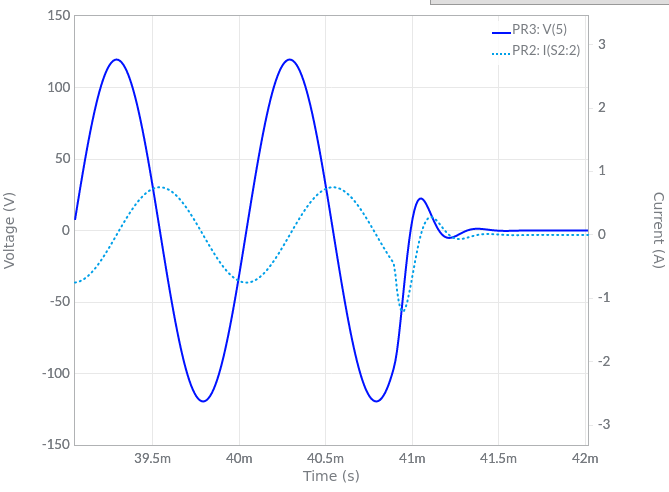
\includegraphics[width=\textwidth]{42}
		\end{minipage}
		\caption{Перехідний процес на конденсаторі.}
	\end{figure}	

	\begin{figure}[H]
		\centering
		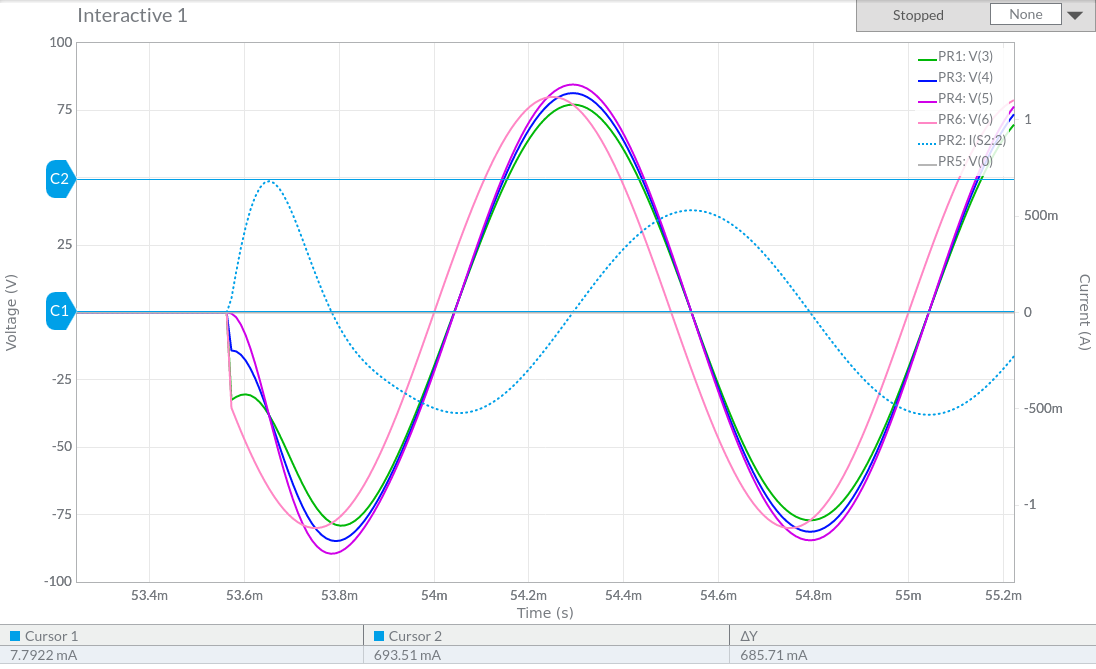
\includegraphics[width=\textwidth]{111}
		\caption{Максимальне відхилення сили струму 0.7 А.}
	\end{figure}

	\begin{figure}[H]
		\centering
		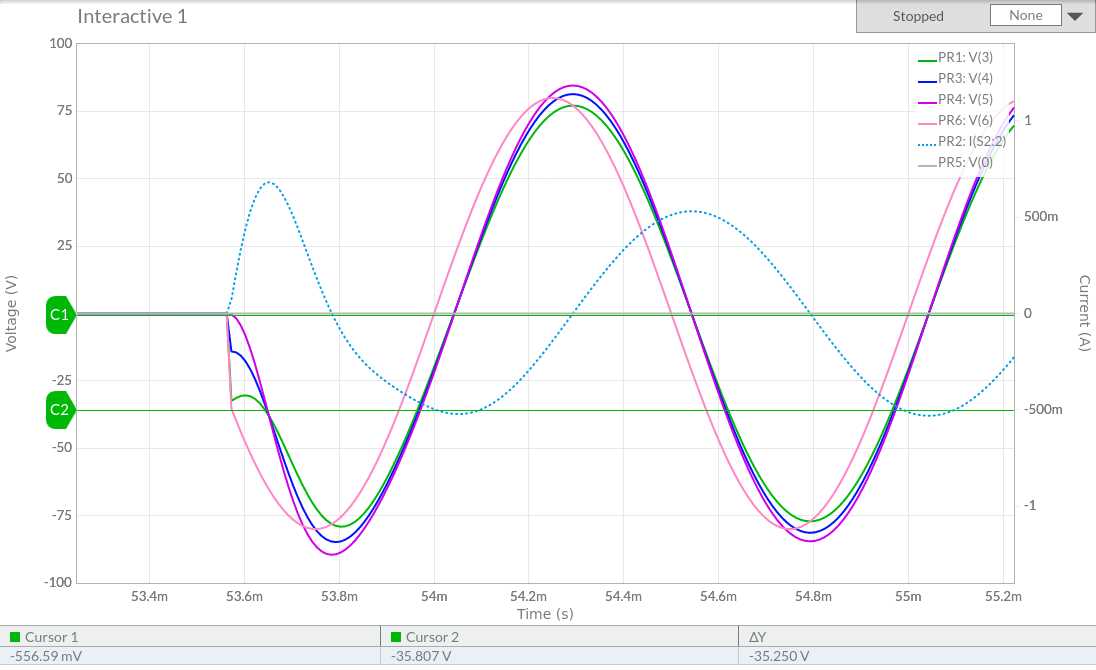
\includegraphics[width=\textwidth]{112}
		\caption{Максимальне відхилення напруги 36 В.}
	\end{figure}

	\begin{figure}[H]
		\centering
		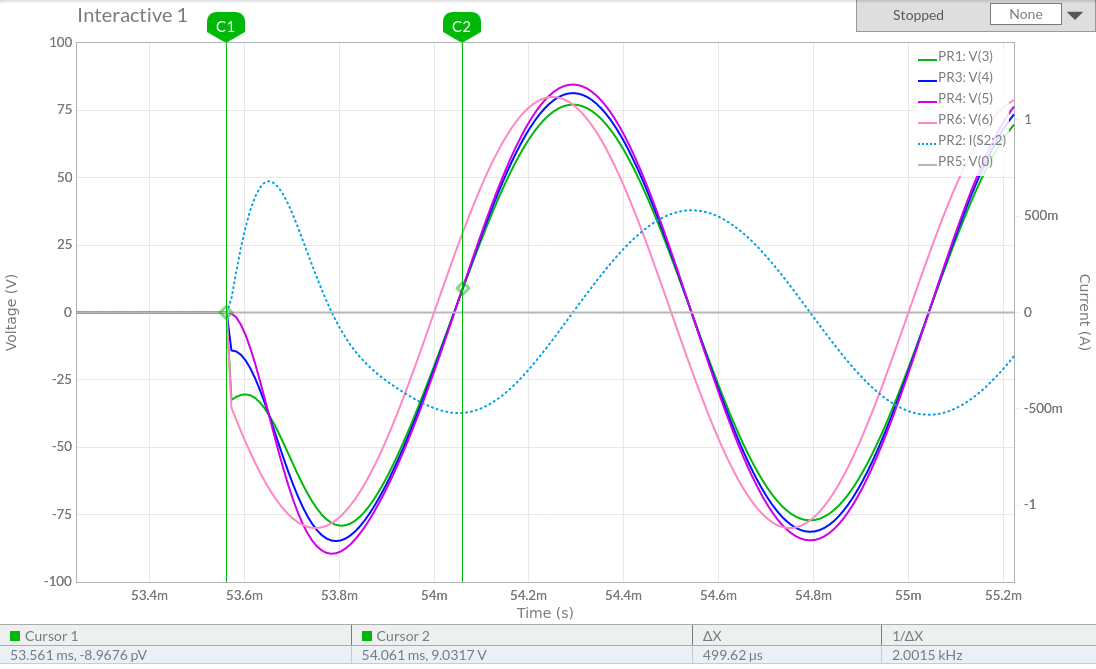
\includegraphics[width=\textwidth]{113}
		\caption{Час перехідного процесу 0.55 мс.}
	\end{figure}

	\begin{figure}[H]
		\centering
		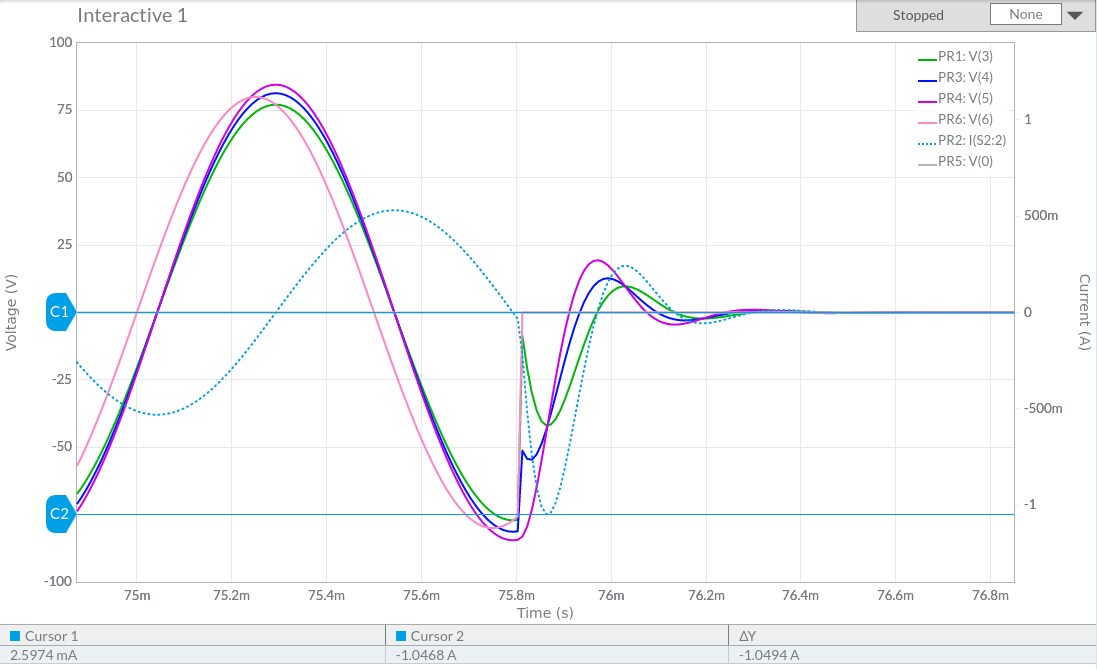
\includegraphics[width=\textwidth]{223}
		\caption{Максимальне відхилення сили струму 1 А.}
	\end{figure}
	
	\begin{figure}[H]
		\centering
		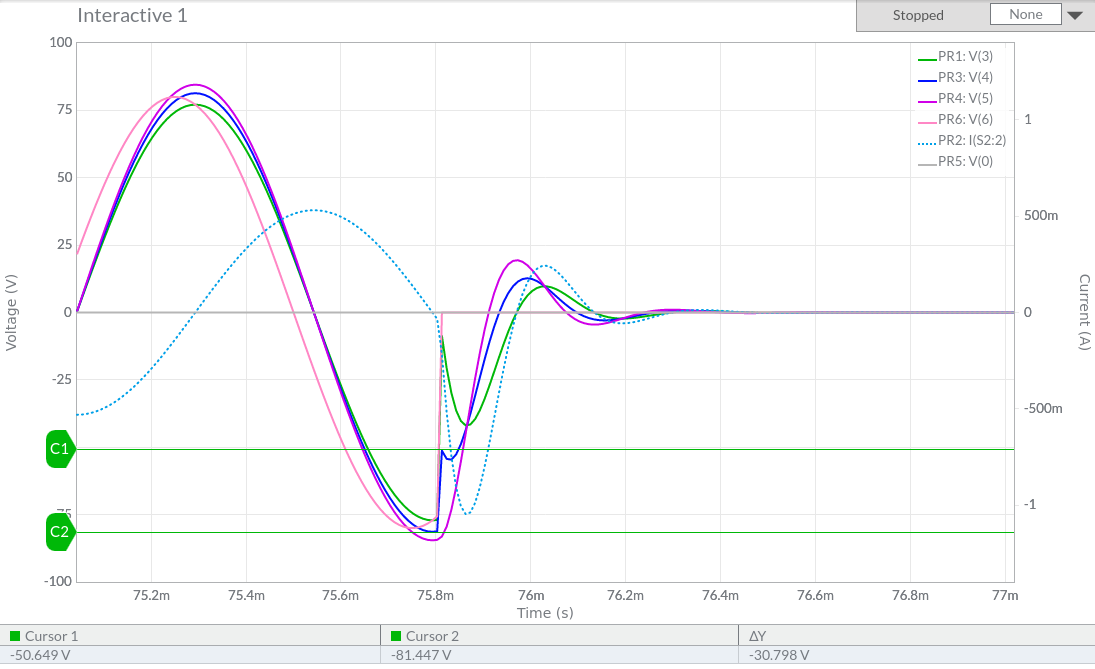
\includegraphics[width=\textwidth]{222}
		\caption{Максимальне відхилення напруги 32 В.}
	\end{figure}
	
	\begin{figure}[H]
		\centering
		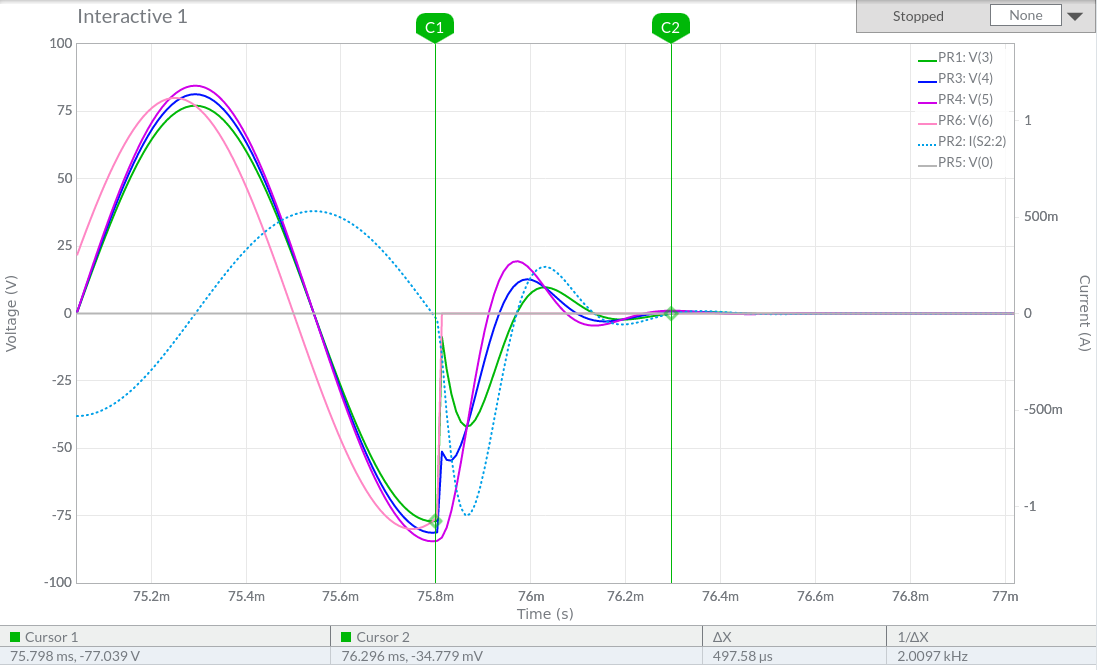
\includegraphics[width=\textwidth]{221}
		\caption{Час перехідного процесу 0.5 мс.}
	\end{figure}

	\begin{figure}[H]
		\centering
		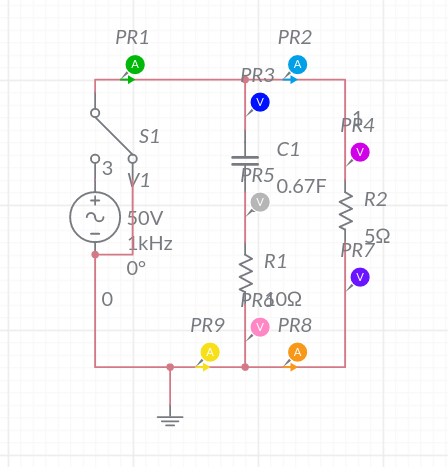
\includegraphics[scale=0.5]{s2}
		\caption{Відтворив схему розгалуженого кола змінного стуму в середовищі Multisim Live.}
	\end{figure}
	
	\begin{figure}[H]
		\centering
		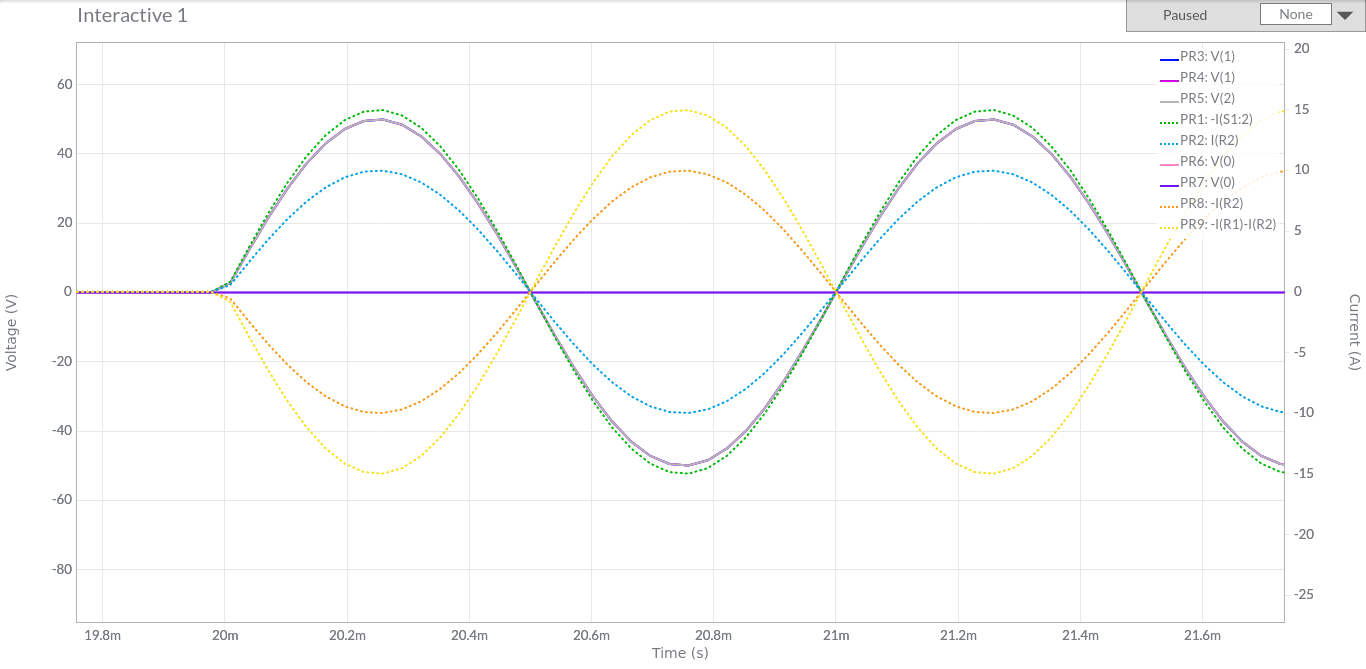
\includegraphics[width=\textwidth]{331}
		\caption{Через відсутність у колі котушки індуктивності відсутні яскраво виражені перехідні процеси.}
	\end{figure}

	\begin{figure}[H]
		\centering
		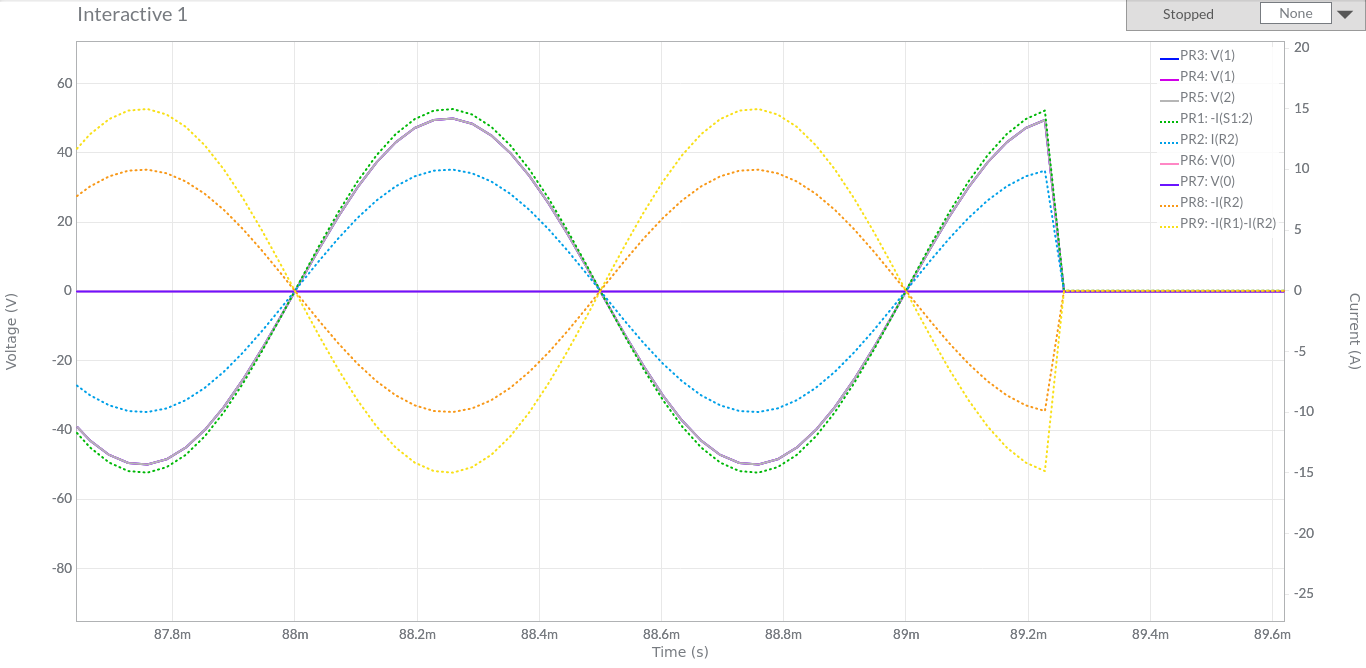
\includegraphics[width=\textwidth]{332}
		\caption{Через відсутність у колі котушки індуктивності відсутні яскраво виражені перехідні процеси.}
	\end{figure}
	
	\section*{Висновки}
	Під час виконання лабораторної роботи я проаналізував перехідні процеси у колах із зосередженими параметрами засобами програмного продукту Multisim Live.
	Навчився обраховувати тривалість перехідних процесів нерозгалуженого та
	розгалуженого кола змінного струму.
	    
\end{normalsize}
\end{document}
